% learning/parsing_em.tex

\marginnote{beginning of parsing\_em.tex}

\def\ind{\mathbf{1}}
\newcommand\Inner{\mathbb{I}}
\newcommand\Outer{\mathbb{O}}
\newcommand\Full{\mathbb{F}}
% \DeclareMathOperator*\Inner{Inner}
% \DeclareMathOperator*\Outer{Outer}
% \DeclareMathOperator*\Full{Full}

\section{Parse trees and Inference}
\marginnote{Add more friendly and/or explanatory text, and examples}

Given a placed symbol $X_{p,q}$, the PCFSG defines a distribution over
concrete substitution rules that can be applied:
\begin{align*}
  P_{sub}( \langle X_{p,q} \to Y_{p,m} Z_{m,q}\rangle ; X_{p,q})
  &= \rho_X([X\to YZ]) \cdot \mu_{X\to YZ}(m; p,q)\\
  P_{sub}( \langle X_{p,q} \to \ell_{p,q} \rangle ; X_{p,q}) 
  &= \rho_X([X\to \ell]).
\end{align*}

We can then define $P(C; \GGG, p,q)$ to be the probability that we
arrive at $C$ by starting with $S_{p,q}$ and repeatedly applying a
random concrete substitution rule according to $P_{sub}$. For a fixed
grammar $\GGG$ and a given curve $C$ with points $C[0], \dots, C[n]$,
there are potentially many ways for this sampling process to produce
$C$. In this section, we formalize this by defining parse trees.

\subsection{Preliminaries}

\begin{defn}
We define the set $\FFF_\GGG$ to be the set of all strings of placed
symbols $X^{(1)}_{p_0,p_1} X^{(2)}_{p_1,p_2} \dots X^{(k)}_{p_{k-1},
  p_k}$ with $X^{(i)} \in \NNN$, where neighboring placed symbols
$X^{(i)}_{p_{i-1},p_i} X^{(i+1)}_{p_i,p_{i+1}}$ are constrained to
share the point $p_i$.
\end{defn}

\marginnote{This probably wants a figure}
Let $C$ be a curve of length $n$, with points $C[0]$ through
$C[n]$. Since $C$ is fixed, we will abuse notation throughout this
section by writing placed symbols $X_{C[i],C[j]}$ as $X_{ij}$.

We will write a binary tree with root node $v$, left subtree $T_1$,
and right subtree $T_2$ as $\frac{v}{T_1\qquad \mid \qquad T_2}.$

\begin{defn}
  Let $T_1, T_2$ be labeled binary trees, where $u$ is a leaf node of
  $T_1$ and $v$ is the root node of $T_2$. We define a new tree $T_1
  \triangle^{\cancel{u}}_v T_2$ to be the tree resulting from deleting
  $u$ and attaching $T_2$ in its place.
\end{defn}

In order to differentiate between abstract and concrete substitutions
we will write the former as $[X\to YZ]$ or $[X\to \ell]$ and the
latter as $\langle X_{ik} \to Y_{ij} Z_{jk} \rangle$ or $\langle X_{i
  i+1} \to \ell_{i i+1} \rangle$.

\subsection{Parse Trees}

\begin{defn}
  A $\GGG$-parse tree is a binary tree $T$ that specifies a set
  of concrete substitution rules that take a placed symbol $X_{ij}$
  to some placed curvilinear form $\lambda$.

  $T$ has three kinds of nodes:
  \begin{itemize}
  \item Unexpanded nodes, which are labeled with a placed symbol
    $X_{ij}$, where $0\le i < j \le n$ and $X\in \NNN$. Unexpanded
    nodes are always leaves.
  \item Lexical nodes, which are labeled with a concrete substitution
    rule $$\langle X_{i i+1} \to \ell_{i i+1}\rangle,$$ where $[X\to \ell]\in
    \RRR(X)$, $X\in \NNN, 0\le i < n$. Lexical nodes are always leaves.
  \item Binary nodes, which are labeled with a concrete substitution
    rule $$\langle X_{ik}\to Y_{ij} Z_{jk}\rangle,$$ where $X,Y,Z\in
    \NNN, [X\to YZ]\in \RRR(X)$, and $0 \le i < j < k \le n$. Binary
    nodes always have two children. The first must be either of the
    form $\langle Y_{ij} \to \lambda \rangle$ or of the form $Y_{ij}$.
    The second must be either of the form $\langle Z_{jk} \to \lambda
    \rangle$ or of the form $Z_{jk}$.
  \end{itemize}
\end{defn}
For brevity, we will refer to $\GGG$-parse trees simply as parse
trees.

To simplify notation, we will define $sym(v)$ as:
\begin{itemize}
\item $sym(X_{ij}) = X_{ij}$
\item $sym(\langle X_{i i+1} \to \ell_{i i+1}\rangle) = X_{i i+1}$
\item $sym(\langle X_{ik} \to Y_{ij} Z_{jk}\rangle) = X_{i k}$
\end{itemize}

\marginnote{Depict a derivation graphically}
We have defined parse trees to represent derivations according to the
substitution rules of $\GGG$.  For $X\in \NNN, p,q\in \RR^2$, the set
of all $\GGG$-parse trees $T$ such that $sym(root(T)) = X_{p,q}$ is in
one-to-one correspondence with the set of all derivations of placed
curvilinear forms from the placed symbol $X_{p,q}$. Unexpanded nodes
correspond to incomplete derivations, while lexical and binary nodes
correspond to applications of lexical and binary substitution
rules. The constraints on the children of binary nodes require that
our derivation then operate on the placed symbols produced by the
substitution rule.

\begin{defn}
The \emph{weight} of a parse tree $T$ is defined to be
$$ W_\GGG(T) = \prod_{\langle X_{ij} \to \lambda \rangle\in T} P_{sub}(
\langle X_{ij} \to \lambda \rangle).$$ Note that this product omits
the unexpanded nodes of $T$.
\end{defn}

The weight of a parse tree multiplies the probability of each concrete
substitution in the parse tree.  We call it a weight rather than a
probability because two different parse trees are not always mutually
exclusive events (in particular, if one is a subset of the other), and
thus $W_\GGG(T)$ does not sum to one over the set of all parse trees.

\begin{obs}
Let $T_1$ be a parse tree with an unexpanded leaf node $X_{ij}$, and let
$T_2$ be a parse tree with root node of the form $\langle X_{ij} \to
\lambda \rangle$. If we define
$$T = T_1 \triangle^{\cancel{X_{ij}}}_{\langle X_{ij} \to \lambda
  \rangle} T_2,$$
then
\begin{enumerate}
\item $T$ is a valid parse tree.
\item $W_\GGG(T) = W_\GGG(T_1) W_\GGG(T_2).$
\end{enumerate}
\end{obs}

\subsection{Inner Parse Trees}

\marginnote{Picture of inner parse tree}
\begin{defn}
  An \emph{inner parse tree} of $C$ is a parse tree $T$ in which every
  leaf node is a lexical node. Let $\Inner_\GGG^C(X_{ij}, \lambda)$ be
  the set of all inner parse trees of $C$ with root node of the form
  $\langle X_{ij} \to \lambda \rangle$. Let $\Inner_\GGG^C(X_{ij})$ be
  the set of all inner parse trees of $C$ with root node of the form
  $\langle X_{ij} \to \lambda \rangle$ for any $\lambda \in \FFF_\GGG$.
\end{defn}

\marginnote{Figure to illustrate this prop}
\begin{prop}
\label{prop-induct-inside}
We can construct the set $\Inner_\GGG^C(X_{ij}, \lambda)$ recursively
as follows:
\begin{itemize}
\item $\Inner_\GGG^C(X_{i i+1}, \ell_{i i+1}) = \left\{ \frac{ \langle
      X_{i i+1} \to \ell_{i i+1} \rangle}{ \emptyset \qquad \mid
      \qquad \emptyset } \right\}$
if $[X\to \ell] \in \RRR(X)$, and empty otherwise.
\item 
$    \Inner_\GGG^C(X_{ij}, Y_{ik} Z_{kj}) = \Bigg\{ \frac{\langle
  X_{ij} \to Y_{ik}Z_{kj} \rangle}{ T_Y \qquad \mid \qquad T_Z} : 
 T_Y\in
      \Inner_\GGG^C(Y_{ik}), T_Z \in \Inner_\GGG^C(Z_{kj}) \Bigg\}.
$
\end{itemize}
\end{prop}
\begin{proof}
  Let $T\in \Inner_\GGG^C(X_{ij})$. The root node is either of the
  form $\langle X_{i i+1} \to \ell_{i i+1}\rangle$ or $\langle X_{i
    j}\to Y_{i k} Z_{k j}\rangle$. In the former case, the root is a lexical
  node, and cannot have any children.

  In the latter case, since $T$ is an inner parse tree, the root node
  cannot be a leaf node, and it is constrained to have exactly two
  children, which must be of the form $\langle Y_{ik}\to
  \lambda_Y\rangle$ and $\langle Z_{kj} \to \lambda_Z \rangle$, since
  $T$ has no unexpanded nodes. Every leaf node of either subtree is
  also a leaf node of $T$, and thus lexical. Therefore the subtrees
  headed by these nodes are also inner parse trees, and reside in the
  specified sets.
\end{proof}

\begin{prop}
\label{prop-inside-corr}
  The set $\Inner_\GGG^C(X_{ij})$ is in one-to-one correspondence with
  the set of derivations of $C[i:j]$ from the placed symbol $X_{ij}$
  according to the substitution rules of $\GGG$. Moreover, $W_\GGG(T)$
  gives the probability of the derivation.
\end{prop}
\begin{proof}
Since inner parse trees cannot have unexpanded nodes, they correspond
to complete derivations of a subcurve from the placed symbol
$X_{ij}$. Since each step of the derivation is chosen independently
from the others, the probability of the parse tree is the product of
the probabilities of the individual substitutions, which is given by $W_\GGG(T)$.
\end{proof}

The probability that we derive a curve $C[i:j]$ from a placed symbol
$X_{ij}$ is just the sum of the probabilities of any particular
derivation, taken over all possible derivations. This probability is
called the \emph{inside probability}:
$$Inside_\GGG^C(X_{i j}) =  \sum_{T\in \Inner_\GGG^C(X_{ij})}W_\GGG(T).$$
Since $P(C\mid \GGG)$ is just the total probability of deriving $C$
from $\GGG$, it is clear by Proposition \ref{prop-inside-corr} that 
$$P(C\mid \GGG) = Inside_\GGG^C(S_{0 n}).$$

We can compute the inside probability efficiently:

\begin{obs}
\label{obs-inside-rec}
We can compute all inside probabilities in time $O(|\RRR|n^3)$ by using the
following relations:
  \begin{align*}
Inside_\GGG^C(X_{i i+1}) &= \sum_{T\in \Inner_\GGG^C(X_{i i+1})}
W_\GGG(T)\\
 &= P_{sub}(\langle X_{i i+1} \to \ell_{i i+1} \rangle) \\
\intertext{by the first case of Proposition \ref{prop-induct-inside}.}
Inside_\GGG^C(X_{ij}) &= \sum_{T\in \Inner_\GGG^C(X_{ij})} W_\GGG(T)\\
&= \sum_{\substack{[X\to YZ] \in \RRR(X)\\ i < k < j}} \sum_{T\in
  \Inner_\GGG^C(X_{ij}, Y_{ik}Z_{kj})} W_\GGG(T)\\
\intertext{by the definition of $\Inner_\GGG^C(X_{ij})$}
&= \sum_{\substack{[X\to YZ] \in \RRR(X)\\ i < k < j}} 
P_{sub}(\langle X_{ij} \to Y_{ik} Z_{kj} \rangle)
\sum_{T_Y\in \Inner_\GGG^C(Y_{ik})}
\sum_{T_Z\in \Inner_\GGG^C(Z_{kj})}
 W_\GGG(T_Y) W_\GGG(T_Z)\\
\intertext{by the second case of Proposition \ref{prop-induct-inside}}
&= \sum_{\substack{[X\to YZ] \in \RRR(X)\\ i < k < j}} 
P_{sub}(\langle  X_{ij} \to Y_{ik} Z_{kj} \rangle)
Inside_\GGG^C(Y_{ik})
Inside_\GGG^C(Z_{kj})
  \end{align*}
\end{obs}

\subsection{Outer Parse Trees}

\marginnote{Picture of outside tree}
\begin{defn}
  An \emph{outer parse tree} of $C$ is a parse tree $T$ with
  $sym(root(T)) = S_{0n}$ in which one special leaf is an unexpanded node
  $X_{ij}$, and all other leaf nodes are lexical nodes. Let
  $\Outer_\GGG^C(X_{ij})$ be the set of all outer parse trees which
  have unexpanded node $X_{ij}$.
\end{defn}

\marginnote{Figure to illustrate this prop}
\begin{prop}
\label{prop-outer-set}
  We can construct the set $\Outer_\GGG^C(X_{ij})$ recursively as
  follows:
\begin{itemize}
\item $\Outer_\GGG^C(X_{0n}) = \left\{ \frac{S_{0n}}{\emptyset \qquad
      \mid \qquad \emptyset} \right\}$, if $X=S$, and is empty otherwise.
\item 
\begin{align*}
&\Outer_\GGG^C(X_{ij}) = \\
&\bigcup_{\substack{h < i \\ [Z \to YX]\in \RRR}}
\Bigg\{
T_{out} \triangle^{\cancel{Z_{hj}}}_{\langle Z_{hj} \to Y_{hi}
  X_{ij})\rangle} \frac{ \langle Z_{hj} \to Y_{hi}
  X_{ij} \rangle}{ T_Y \qquad \mid \qquad X_{ij}} : \\
&\qquad\qquad\qquad T_{out} \in \Outer_\GGG^C(Z_{hj}), T_Y \in \Inner_\GGG^C(Y_{hi}) 
\Bigg\} \bigcup\\
&\bigcup_{\substack{i < k \\ [Z \to
    XY]\in \RRR}}
\Bigg\{
T_{out} \triangle^{\cancel{Z_{ik}}}_{\langle Z_{ik} \to X_{ij} Y_{jk}
  \rangle} \frac{ \langle Z_{ik} \to X_{ij}
  Y_{jk} \rangle}{ X_{ij} \qquad \mid \qquad  T_Y } :\\
&\qquad\qquad\qquad T_{out} \in \Outer_\GGG^C(Z_{ik}),
 T_Y \in \Inner_\GGG^C(Y_{jk}) \Bigg\}\\
\end{align*}
(For notational simplicity above, we are writing $X_{ij}$ in
place of $\frac{X_{ij}}{\emptyset \qquad \mid \qquad
  \emptyset}$.)
\end{itemize}
\end{prop}
\begin{proof}
  Let $T\in \Outer_\GGG^C(X_{ij})$. The unexpanded
  node $X_{ij}$ may be the root of $T$, in which case $X_{ij}$ must be
  $S_{0n}$, and we are in the first case.

  Otherwise, $X_{ij}$ is not the root of $T$, and has a parent which
  is either $\langle Z_{hj} \to Y_{hi} X_{ij} \rangle$, or $\langle
  Z_{ik} \to X_{ij} Y_{jk} \rangle$. Let us restrict to the second
  case; the first case is strictly analogous. 
  
  If we remove the subtree rooted at $Y_{jk}$ and replace $\langle
  Z_{ik} \to X_{ij} Y_{jk} \rangle$ with an unexpanded node $Z_{ik}$, we get a
  tree $T_{out}$ which is a valid outer tree for $Z_{ik}$:
  \begin{itemize}
  \item $T_{out}$ has a single unexpanded node $Z_{ik}$
  \item $root(T_{out}) = root(T) = S_{0n}$.
  \end{itemize}
  Furthermore, the subtree $T_Y$ rooted at $Y_{jk}$ satisfies
  $sym(root(T_Y)) = Y_{jk}$, and is an inner parse tree, since all
  remaining leaf nodes are lexical nodes. This completes the proof.
  
\end{proof}

We define the \emph{outside weight} as:
$$Outside_\GGG^C(X_{ij}) = \sum_{T\in \Outer_\GGG^C(X_{ij})}
W_\GGG(T).$$ This gives the total weight of parse trees corresponding
to derivations of the curvilinear form $\ell_{C[0], C[1]}\dots
\ell_{C[i-1],C[i]} X_{ij} \ell_{C[j], C[j+1]} \dots \ell_{C[n-1],
  C[n]}$ from $S_{0n}$.

\begin{obs}
\label{obs-outside-rec}
  Given the inside probabilities, we can compute the outside weights
  in time $O(|\RRR| n^3)$ by using the following relations:
  \begin{align*}
    Outside_\GGG^C(S_{0n}) &= \sum_{T\in \Outer_\GGG^C(S_{0n})}
    W_\GGG(T) \\
&= W_\GGG\left(\frac{S_{0n}}{\emptyset \qquad \mid \qquad
    \emptyset}\right) = 1\\
\intertext{by the first case of Proposition \ref{prop-outer-set}.}
Outside_\GGG^C(X_{ij}) 
&= \sum_{T\in \Outer_\GGG^C(X_{ij})}
    W_\GGG(T) \\
&=
 \sum_{\substack{h < i \\ [Z\to YX] \in
    \RRR}} P_{sub}(\langle Z_{hj} \to Y_{hi}X_{ij} \rangle)
\sum_{T_{out}\in \Outer_\GGG^C(Z_{hj})}
\sum_{T_{Y}\in \Inner_\GGG^C(Y_{hi})}
W_\GGG(T_{out}) W_\GGG(T_Y)\\
&+
 \sum_{\substack{j<k \\ [Z\to XY] \in
    \RRR}} P_{sub}(\langle Z_{ik} \to X_{ij}Y_{jk} \rangle)
\sum_{T_{out}\in \Outer_\GGG^C(Z_{ik})}
\sum_{T_{Y}\in \Inner_\GGG^C(Y_{jk})}
W_\GGG(T_{out}) W_\GGG(T_Y)
\intertext{by the second case of Proposition \ref{prop-outer-set}.}
&= 
 \sum_{\substack{h < i \\ [Z\to YX] \in
    \RRR}} P_{sub}(\langle Z_{hj} \to Y_{hi}X_{ij} \rangle)
Outside_\GGG^C(Z_{hj}) Inside_\GGG^C(Y_{hi})\\
&+
 \sum_{\substack{j<k \\ [Z\to XY] \in
    \RRR}} P_{sub}(\langle Z_{ik} \to X_{ij}Y_{jk} \rangle)
Outside_\GGG^C(Z_{ik}) Inside_\GGG^C(Y_{jk})
  \end{align*}
\end{obs}

\subsection{Dealing with Closed Curves}

When we are dealing with a closed curve $C$, the machinery of the
preceding sections does not work as is. Rather than using $S_{0n}$
to represent the whole curve, we have $S_{00}$, since $C[n-1]$ is
connected to $C[0]$. Moreover, there is no reason why parse trees
should necessarily be rooted at $S_{00}$, since we can split the curve
at an index other than $0$.

In order to allow a curve to be split in other ways, we define a
rotation operation:
$$C^{\leftarrow k}[i] = C[(i-k) \mod n].$$
We think of $C$ as being a random rotation of some other closed
curve $D$, and set $P(C = D^{\leftarrow k}) = \frac{1}{n}$.

%% We can then treat the closed curve $D[0], \dots, D[n-1]$ as an open
%% curve $D[0], \dots, D[n-1], D[n]=D[0]$ whose endpoints happen to be
%% the same.

\begin{rmk}
  For closed curve grammars, the top-level midpoint distributions
  $\mu_{S\to XY}$ cannot be proper distributions if our grammar is
  going to be invariant under similarity transformations (translation,
  scaling, and rotation). This is because any choice of midpoint is
  equally good, since we can map any pair $(p,q)$ to any other pair
  $(p',q')$ via a similarity transformation. This is a problem
  because we cannot define a uniform distribution on all of $\RR^2$!

  We handle this by setting $\mu_{S\to XY}(\cdot) = 1$ in our
  formulas. We justify this by thinking of each curve as being a
  representative of its equivalence class under similarity
  transformations.  
\end{rmk}

The probability that we see a parse tree is therefore $P(C,T\mid \GGG)
= \frac{1}{n} W_\GGG(T).$ In order to describe the parse trees, we
must allow placed symbols $X_{ij}$, where $j<i$. In this case,
$X_{ij}$ will be understood to be a placed symbol that ultimately
expands to be all the indices between $0$ and $n$ that are after $i$
or before $j$. To simplify matters, we introduce clockwise intervals:

\begin{marginfigure}
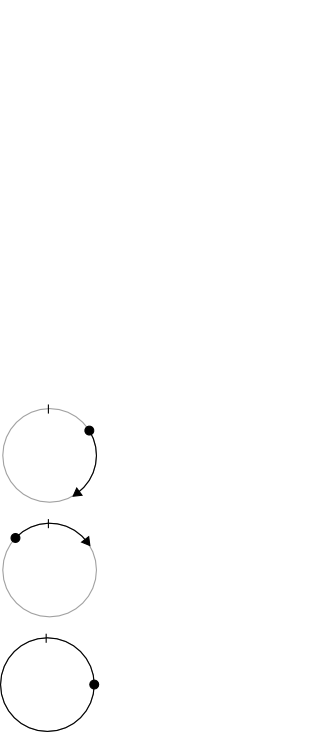
\includegraphics[width=\linewidth]{figures/circular_intervals/cw.png}
\caption{The three kinds of clockwise intervals.}
\end{marginfigure}
$$cw_n(i,j) = 
\begin{cases}
\{k \in \ZZ \mid i < k < j\} & i < j \\
\{k \in \ZZ \mid 0 \le k < j \mbox{ or } i < k < n \} & i > j \\
\{k \in \ZZ \mid 0\le k < n, k\ne i \} & i = j\\
\end{cases}.$$
These are the indices in between $i$ and $j$ on the curve, where we
move ``clockwise'' in the direction of increasing indices.  We also
introduce counter-clockwise intervals
\begin{marginfigure}
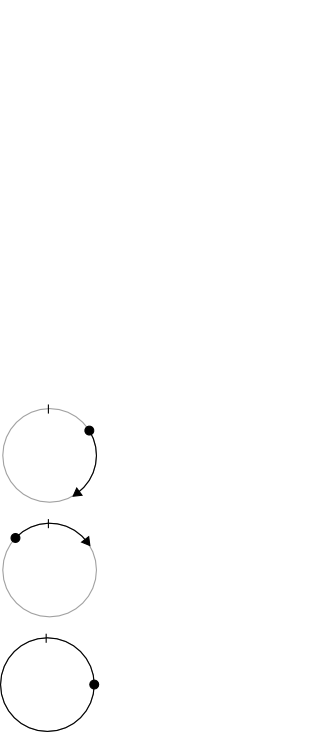
\includegraphics[width=\linewidth]{figures/circular_intervals/cw.png}
\caption{The three kinds of counter-clockwise intervals.}
\end{marginfigure}
$$ccw_n(i,j) = 
\begin{cases}
\{k \in \ZZ \mid 0 \le k < i \mbox{ or } j < k < n \} & i < j \\
\{k \in \ZZ \mid j < k < i\} & i > j \\
\emptyset & i = j\\
\end{cases}.$$
These are the points which are outside of the clockwise interval
between $i$ and $j$, excluding $i$ and $j$.

We can then adapt Observations \ref{obs-inside-rec} and \ref{obs-outside-rec} as follows:

\begin{prop}
We can recursively compute inside weights in time $O(|\RRR| n^3)$:

\begin{align*}
CInside_\GGG^C(X_{i i+1}) &= P_{sub} (\langle X_{ii+1} \to \ell_{i i+1}\rangle) \\
CInside_\GGG^C(X_{(n-1)0}) &= P_{sub} (\langle X_{(n-1)0} \to \ell_{(n-1)0}\rangle) \\
CInside_\GGG^C(X_{ij}) &= \sum_{\substack{[X\to YZ]\in \RRR(X)\\ k\in cw_n(i,j)}} 
P_{sub}(\langle X_{ij} \to Y_{ik} Z_{kj}\rangle) CInside_\GGG^C(Y_{ik}) CInside_\GGG^C(Z_{kj}).
\end{align*}
\end{prop}

\begin{prop}
We can recursively compute outside weights in time $O(|\RRR| n^3)$:

\begin{align*}
COutside_\GGG^C(S_{ii}) &= 1\\
COutside_\GGG^C(X_{ij}) &=
\sum_{\substack{h\in ccw_n(i,j) \\ [Z\to YX] \in \RRR}} P_{sub}(\langle Z_{hj} \to Y_{hi} X_{ij} \rangle)
COutside_\GGG^C(Z_{hj}) CInside_\GGG^C(Y_{hi})\\
&+ \sum_{\substack{k \in ccw_n(i,j)\\ [Z\to XY] in \RRR}}
P_{sub}(\langle Z_{ik} \to X_{ij} Y_{jk} \rangle)
COutside_\GGG^C(Z_{ik}) CInside_\GGG^C(Y_{jk}).
\end{align*}
\end{prop}

%% \subsubsection{old stuff about closed curves}

%% The probability that we see a parse tree is therefore $P(C,T\mid \GGG)
%% = \frac{1}{n} W_\GGG(T).$ The inside weights are unaffected by this
%% change - once we specify the root node $X_{ij}$, it is irrelevant
%% which shift of $C$ is being examined. (Although some shifts will not
%% allow $X_{ij}$, since $C[j]$ will be to the left of $C[i]$.)

%% The outside weights are affected by the change. For each $k$ such that
%% $0\le k < n$, we have a distinct $Outside_\GGG^{C^{\leftarrow
%%     k}}(X_{ij})$.
%% We can simplify matters by defining 
%% $$COutside_\GGG^C(X_{ij}) = \frac{1}{n} \sum_k
%% Outside_\GGG^{C^{\leftarrow k}}(X_{(i + k \mod n) (j + k \mod n)}).$$

%% \begin{prop}
%% We can compute $COutside_\GGG^C(X_{ij})$ recursively as follows:
%% $$COutside_\GGG^C(S_{ii}) = \frac{1}{n}.$$

%% \begin{align*}
%% COutside_\GGG^C(X_{ij}) &=
%%    \sum_{\substack{h < i \\ [Z\to YX] \in
%%     \RRR}} P_{sub}(\langle Z_{hi} \to Y_{hi}X_{ij} \rangle)
%% COutside_\GGG^C(Z_{hj}) Inside_\GGG^C(Y_{hi})\\
%% &+
%%  \sum_{\substack{j<k \\ [Z\to XY] \in
%%     \RRR}} P_{sub}(\langle Z_{ik} \to X_{ij}Y_{jk} \rangle)
%% COutside_\GGG^C(Z_{ik}) Inside_\GGG^C(Y_{jk})
%% \end{align*}
%% \end{prop}
%% \begin{proof}
%% \mar{finish and prove by induction.}
%% We proceed by downwards induction on the length of $X_{ij}$. The value
%% for $COutside_\GGG(S_{ii})$ is straight from the definition.

%% \end{proof}

\marginnote{end of parsing\_em.tex}
